\documentclass[
	12pt,				% tamanho da fonte
	openright,			% capítulos começam em pág ímpar (insere página vazia caso preciso)
	oneside,			% para impressão apenas em um lado do papel
	a4paper,			% tamanho do papel.
	brazil				% o último idioma é o principal do documento
	]{abntex2}

% ---
% Pacotes básicos
% ---

\usepackage{etoolbox}
\usepackage{lmodern}			% Usa a fonte Latin Modern
\usepackage[T1]{fontenc}		% Selecao de codigos de fonte.
\usepackage[utf8]{inputenc}		% Codificacao do documento (conversão automática dos acentos)
%\usepackage{lastpage}			% Usado pela Ficha catalográfica
\usepackage{indentfirst}		% Indenta o primeiro parágrafo de cada seção.
\setlength{\parindent}{1.5cm}   % Espaçamento de 1,5cm do parágrafo
\usepackage{color}				% Controle das cores
\usepackage{graphicx}			% Inclusão de gráficos
\usepackage{microtype} 			% para melhorias de justificação
\usepackage{lipsum}				% para geração de dummy text
\usepackage[alf]{abntex2cite}	% Citações padrão ABNT
\usepackage[table,xcdraw]{xcolor}% Cédula colorida em tabelas
\usepackage{pdflscape}          % Rotaciona página
% \usepackage{Capa}               % Capa e folha de rosto com modificações
\usepackage{float}              % Melhor posicionamento de figuras
\usepackage{gensymb}            % símbolo º
\usepackage[justification=justified,singlelinecheck=false]{caption}
%\usepackage{etoolbox}           % Configurações adicionais de macros
\usepackage{xparse}
\usepackage{multirow}
\NewDocumentCommand\cc{+u{\cc}}{\ignorespaces}

\usepackage{amsmath, amssymb, amsthm}

% -----------------------------------------------------------------------
\renewcommand{\imprimircapa}{%
  \begin{capa}%
    \center
    \ABNTEXchapterfont\Large \imprimirinstituicao \\
    \vspace*{1cm}
    {\ABNTEXchapterfont\large\imprimirautor}
    \vfill
    \ABNTEXchapterfont\bfseries\LARGE\imprimirtitulo
    \vfill
    \large\imprimirlocal
    \par
    \large\imprimirdata
    \vspace*{1cm}
  \end{capa}
}


\makeatletter
\renewcommand{\folhaderostocontent}{
  \begin{center}
    {\ABNTEXchapterfont\large\imprimirautor}
    \vspace*{\fill}\vspace*{\fill}
    \begin{center}
      \ABNTEXchapterfont\bfseries\Large\imprimirtitulo
    \end{center}
    \vspace*{\fill}
    \abntex@ifnotempty{\imprimirpreambulo}{%
      \hspace{.45\textwidth}
      \begin{minipage}{.5\textwidth}
        \SingleSpacing
        \imprimirpreambulo \hfill
      \end{minipage}%
      \vspace{0.5cm}

      \hspace{.45\textwidth}
      \begin{minipage}{.5\textwidth}
        \imprimirorientadorRotulo~\imprimirorientador \hfill
      \end{minipage}%
      \vspace*{\fill}
    }%
    \vfill
    {\large\imprimirlocal}
    \par
    {\large\imprimirdata}
    \vspace*{1cm}
  \end{center}
}
\makeatother
%-----------------------------------------------------------------------



% ---
% Dados dos documento
% ---

\titulo{FATORES DE RISCO PARA O ÓBITO POR HANTAVIROSE NO PARANÁ, 1992-2016, UMA ABORDAGEM POR UM MODELO DE FRAÇÃO DE CURA.}
% \autor{Nome Aluno 1 \\ Nome Aluno 2}
\autor{Pedro Henrique Pavan Gonçalves \\ }
\data{2022}
\instituicao{Universidade Federal do Paraná
             \par
             Setor de Ciências Exatas
             \par
             Departamento de Estatística
%             \par
%             Curso de Estatística
            }
\local{Curitiba}
\orientador[Orientador(a):]{Silvia Emiko Shimakura}
\preambulo{Trabalho de Conclusão de Curso apresentado à disciplina Laboratório B do Curso de Graduação em Estatística da Universidade Federal do Paraná, como exigência parcial para obtenção do grau de Bacharel em Estatística.}

% ---
% Configurações básicas
% ---

% informações do PDF

\makeatletter
\hypersetup{
     	%pagebackref=true,
  pdftitle={\@title},
  pdfauthor={\@author},
  pdfsubject={\imprimirpreambulo},
  colorlinks=true,       		% false: boxed links; true: colored links
  linkcolor=black,          	% color of internal links
  citecolor=black,            % color of links to bibliography
  filecolor=magenta,      	% color of file links
  urlcolor=black,
  bookmarksdepth=4
}
\makeatother

\setlength\afterchapskip{\lineskip}

% ----
% Início do documento
% ----

\begin{document}
\frenchspacing     % Retira espaço extra obsoleto entre as frases.

% ----------------------------------------------------------
% ELEMENTOS PRÉ-TEXTUAIS
% ----------------------------------------------------------

% ---
% Capa
% ---
\imprimircapa
% ---

% ---
% Folha de rosto
% ---
\imprimirfolhaderosto
% ---

\begin{dedicatoria}  % Opcional
  \vspace*{\fill}
  Dedico à fulano\ldots{}
  \vspace*{\fill}
\end{dedicatoria}

% --------------
% Agradecimentos  % Opcional
% --------------

\begin{agradecimentos}
  \bigskip
  Agradeço a mim mesmo e a todos que me ajudaram.

Agradeço também a todo mundo que me ajudou e também aos que não me
ajudaram, pois eles também me ajudaram.
\end{agradecimentos}

\begin{epigrafe} % Opcional
  \vspace*{\fill}
  \begin{flushright}
    \emph{Democracia é oportunizar a todos o mesmo ponto de partida.}

\emph{Quanto ao ponto de chegada, depende de cada um.}

Fernando Sabino.
  \end{flushright}
\end{epigrafe}

% ------
% Resumo
% ------
\newpage
\setlength{\absparsep}{18pt}   % ajusta o espaçamento dos parágrafos do resumo
\setlength{\abstitleskip}{1cm} % adiciona mais um cm após o 'titulo' do Resumo para ficar com 2cm,

\begin{resumo}
  \SingleSpacing
  O resumo deve ser escrito em apenas um parágrafo, e deve ser bastante
  chamativo para fazer com que o leitor tenha interesse em prosseguir com
  a leitura. Um bom resumo é sucinto e ao mesmo tempo empolgante. O resumo
  deve conter um pouico de cada parte do texto, mas deve enfatizar aquilo
  que é novidade e os principais resultados obtidos.

  \textbf{Palavras-chave}:
    Palavra-chave 1.
    Palavra-chave 2.
  \end{resumo}

% ---
% inserir o sumario
% ---
\pdfbookmark[0]{\contentsname}{toc}
\tableofcontents*
\cleardoublepage
% ---

\makepagestyle{abntheadings}
\makeevenhead{abntheadings}{\ABNTEXfontereduzida\thepage}{}{}
\makeoddhead{abntheadings}{}{}{\ABNTEXfontereduzida\thepage}
\makeheadrule{abntheadings}{\textwidth}{0in}

% ----------------------------------------------------------
% ELEMENTOS TEXTUAIS
% ----------------------------------------------------------
\textual

\hypertarget{introduuxe7uxe3o}{%
\chapter{Introdução}\label{introduuxe7uxe3o}}

\bigskip

A hantavirose, zoonose viral aguda, cuja infecção em humanos no Brasil, se apresenta na forma da Síndrome Cardiopulmonar por Hantavírus, apresentou seus primeiros casos registrados em 1993, e desde então diversos outros estados tem sido comfirmados em todas as regiões do país.

Uma zoonose é uma doença infecciosa que saltou de um animal não humano para humanos. Os patógenos zoonóticos podem ser bacterianos, virais ou parasitários, ou podem envolver agentes não convencionais, se espalhando assim para humanos por contato direto ou por meio de alimentos, água ou meio ambiente. Eles representam um grande problema de saúde pública em todo o mundo devido à nossa estreita relação com os animais, seja na agricultura, como companheiros ou no ambiente natural \cite{OMS_zoonoses}.

A transmissão da hantavirose é feita por roedores. O mais comum é que o contágio ocorra diretamente pela inalação de partículas de urina, fezes e saliva de roedores silvestres, não pelo contato com outros humanos infectados. Por isso, os casos da doença costumam ser isolados. Diferentemente dos seres humanos, roedores, como ratos e ratazanas, podem carregar o hantavírus por toda a vida sem adoecer \cite{bbc}.

Quando olhamos os dados relacionados a essa zoonose, de 2007 a 2015, foram notificados 13.181 casos de hantavirose no Brasil, dos quais 8\% (\(N=1,060\)) foram confirmados e 3,1\% (\(N=410\)) evoluíram para óbito. Observou-se uma média de 1.465 casos suspeitos notificados por ano, sendo 2008 (N=1.148) e 2013 (N=1.804) os períodos de menor e maior número de notificações, respectivamente \cite{Para2018}.

Segundo a OMS, não há nenhum tratamento, cura ou vacina para a infecção. A alta taxa de mortalidade e dificuldade com o tratamento são fatores que juntamente com a não descoberta de um tratamento tem aumentado a preocupação com a doença que desafia as autoridades de saúde pública ao redor do mundo. As alternativas terapêuticas para os indivíduos infectados limitam-se à introdução de medidas de suporte na fase aguda em ambiente hospitalar, preferivelmente em UTIs.

Dadas as circunstâncias, este presente trabalho de conclusão de curso tem como finalidade estender o trabalho realizado pela DANIELE AKEMI ARITA (cite dani), utilizando os mesmos dados e buscando analisar a sobrevida desses pacientes diagnosticados com hantavirose.

Dado o fato de que nem todos indivíduos do estudo experimentaram o evento de interesse (isto é, não foram a óbito devido à contaminação da hantavirose) até o termino do estudo, é proposta a utilização do modelo de sobrevivência com fração de cura apresentado por \citeonline{cureModels}, para analisar a sobrevida desses pacientes, onde a variável resposta é o tempo decorrido entre a data do primeiro sintoma do paciente e a data em que o mesmo foi levado a óbito.

\hypertarget{objetivos}{%
\chapter{Objetivos}\label{objetivos}}

\bigskip

\hypertarget{objetivo-geral}{%
\section{Objetivo Geral}\label{objetivo-geral}}

O presente estudo tem como objetivo estudar o tempo até a cura ou óbito, de um paciente infectado Hantavirose no Estado do Paraná no período de 1992 a 2016.

\hypertarget{objetivos-especuxedficos}{%
\section{Objetivos Específicos}\label{objetivos-especuxedficos}}

\begin{enumerate}
\def\labelenumi{\alph{enumi}.}
\tightlist
\item
  Revisar a literatura no que diz respeito às abordagens propostas para Análise de Sobrevivência;
\item
  Revisar os pacotes disponíveis no software R (cite r) para estimação e diagnóstico de uma modelagem usando Análise de Sobrevivência fazendo uso dos pacotes survival (cite survival) e smcure (cite smcure);
\item
  Realizar uma análise descritiva dos dados descritos na Seção 3.1.1 para entendimento mais detalhado e consistente das informações;
\item
  Com base nos dados obtidos do banco de monitoramento da Secretaria de Estado da Saúde do Paraná (SESA/PR), realizar uma modelagem usando Análise de Sobrevivência em busca de definir os fatos causadores do óbito ou cura de um paciente infectado por Hantavirose.
\item
  Apresentar o modelo, discutir os resultados obtidos e tirar conclusões.
\end{enumerate}

\hypertarget{revisuxe3o-de-literatura}{%
\chapter{Revisão de Literatura}\label{revisuxe3o-de-literatura}}

\bigskip

Digite aqui sua revisão de literatura.

Veja como fazer citações na introdução.

\hypertarget{material-e-muxe9todos}{%
\chapter{Material e Métodos}\label{material-e-muxe9todos}}

\bigskip

\hypertarget{material}{%
\section{Material}\label{material}}

\hypertarget{conjunto-de-dados}{%
\subsection{Conjunto de dados}\label{conjunto-de-dados}}

O conjunto de dados composto por 280 indivíduos e 69 variáveis utilizado é proveniente do Sistema de Informação de Agravos de Notificação (SINAN), onde para todos os indivíduos presentes na base, as informações referentes foram retiradas da ficha de investigação, onde cada um dos 69 campos presentes na ficha foram preenchidos manualmente. A ficha de investigação preenchida pelos pancientes foi anexada aos apêndices do trabalho.

A população do estudo compreendeu todos os casos de hantavirose confirmados no estado do Paraná e que apresentaram início dos sintomas dentro do período do estudo (Janeiro de 1992 a Junho de 2016)

Neste trabalho, a variável resposta de interesse tempo (em dias), foi calculada através do tempo entre as datas data de óbito e a data do 1º sintoma do indivíduo conforme a função a seguir.

\[tempo = \text{data óbito} - \text{data primeiro sintoma}\]

Para os indivíduos que não apresentaram data de óbito, o tempo (em dias) foi calculada através do tempo entre as datas data de encerramento e a data do 1º sintoma do indivíduo conforme a função a seguir.

\[tempo = \text{data encerramento} - \text{data primeiro sintoma}\]

Feito isso, os dados foram divididos entre cura e óbito, sendo cura o ``indivíduo notificado por serviço de saúde do Estado do Paraná, no período de estudo e que tenha sido confirmado para hantavirose com evolução para cura'' e óbito, o ``indivíduo notificado por serviço de saúde do Estado do Paraná, no período de estudo e que tenha sido confirmado para hantavirose com evolução para óbito''.

Pacientes que não apresentaram data de óbito foram considerados como censura.

\newpage

\hypertarget{recursos-computacionais}{%
\subsection{Recursos Computacionais}\label{recursos-computacionais}}

O software escolhido para a condução do estudo é o software livre \citeonline{citer}, que será utilizado como ferramenta para a análise exploratória, bem como ajustar os modelos.
Os pacotes survival \citeonline{survival} e smcure \citeonline{smcure} serão utilizados no ajuste dos modelos de Análise de Sobrevivência.

\hypertarget{muxe9todos}{%
\section{Métodos}\label{muxe9todos}}

\hypertarget{anuxe1lise-de-sobrevivuxeancia}{%
\subsection{Análise de Sobrevivência}\label{anuxe1lise-de-sobrevivuxeancia}}

\hypertarget{modelo-de-frauxe7uxe3o-de-cura}{%
\subsection{Modelo de Fração de Cura}\label{modelo-de-frauxe7uxe3o-de-cura}}

\hypertarget{resultados-e-discussuxe3o}{%
\chapter{Resultados e Discussão}\label{resultados-e-discussuxe3o}}

\bigskip

\hypertarget{material-final-do-estudo}{%
\section{Material final do Estudo}\label{material-final-do-estudo}}

A princípio foi realizada uma análise descritiva dos dados visando um maior entendimento da base.

A base de dados original era composta por 280 observações e 69 variáveis, que são elas os 69 campos presentes na ficha de investigação preenchida pelos pacientes.

Após a importação dos dados para o R, logo de cara foi possível notar uma grande presença de dados \emph{missing}, ou seja, uma grande quantidade de dados faltantes para as variáveis. Tendo em vista esse problema, foi decidido que as variáveis que apresentassem dados faltantes seriam retiradas, fazendo assim com que restassem apenas 14 variáveis para a análise. A seguir temos uma breve apresentação das variáveis:

\begin{enumerate}
\def\labelenumi{\arabic{enumi}.}
\tightlist
\item
  Tempo: Tempo decorrido do primeiro sintoma do paciente até o óbito ou perda do acompanhamento.
\item
  Idade: Idade do paciente.
\item
  Sexo: Sexo do paciente (homem ou mulher).
\item
  Tontura: Apresentou tontura (sim ou não).
\item
  Cefaleia: Apresentou cefaleia (sim ou não).
\item
  Sangramento Respiratório: Apresentou sangramento respiratório (sim ou não).
\item
  Dispineia: Apresentou falta de ar (sim ou não).
\item
  Hipotensão: Apresentou problemas com pressão baixa (sim ou não).
\item
  Mialgia: Apresentou dores musculares (sim ou não).
\item
  Regional de Saúde: Regional de saúde na qual o paciente foi atendido, podendo ser União da vitória, Guarapuava, Irati e Outros (sim ou não).
\item
  Sinais Hemorrágicos: Apresentou sinais hemorrágicos (sim ou não).
\item
  Internação: Paciente foi internado no periodo em que esteve com a doença (sim ou não).
\item
  Diarreia: Apresentou diarreia (sim ou não).
\item
  Ureia e Creatina: Aumento de Ureia e Creatina (sim ou não).
\end{enumerate}

Para fins de visualização e melhor intendimento da variável, entendeu-se que seria adequado categorizar a variável \emph{idade}, entre indivíduos de 1 a 20 anos de idade, 20 a 29, 30 a 39, 40 a 49, 50 a 59 e com idade superior a 60 anos.

Conforme já foi discutido anteriormente na seção xxxx, em análise de sobrevivência, as censuras são compostas por indivíduos do estudo que ainda não experimentaram o evento final, portanto, além das 14 variáveis escolhidas que sobraram para a continuação do estudo, ainda foi adicionada a variável de censura, onde o indíviduo que apresentou censura é \emph{1} e \emph{0} para o indivíduo não censurado.

\hypertarget{analise-descritiva}{%
\section{Analise Descritiva}\label{analise-descritiva}}

Inicialmente, foi realizada uma análise descritiva dos dados apresentados na Seção 5.1 a fim de analisar a quantidade de indivíduos em cada categoria das variáveis.

Na figura 1, conseguimos analisar a distribuição e comportamento das variáveis idade e sexo, além das quantidades de censura para cada uma.

\begin{figure}[!h]

{\centering 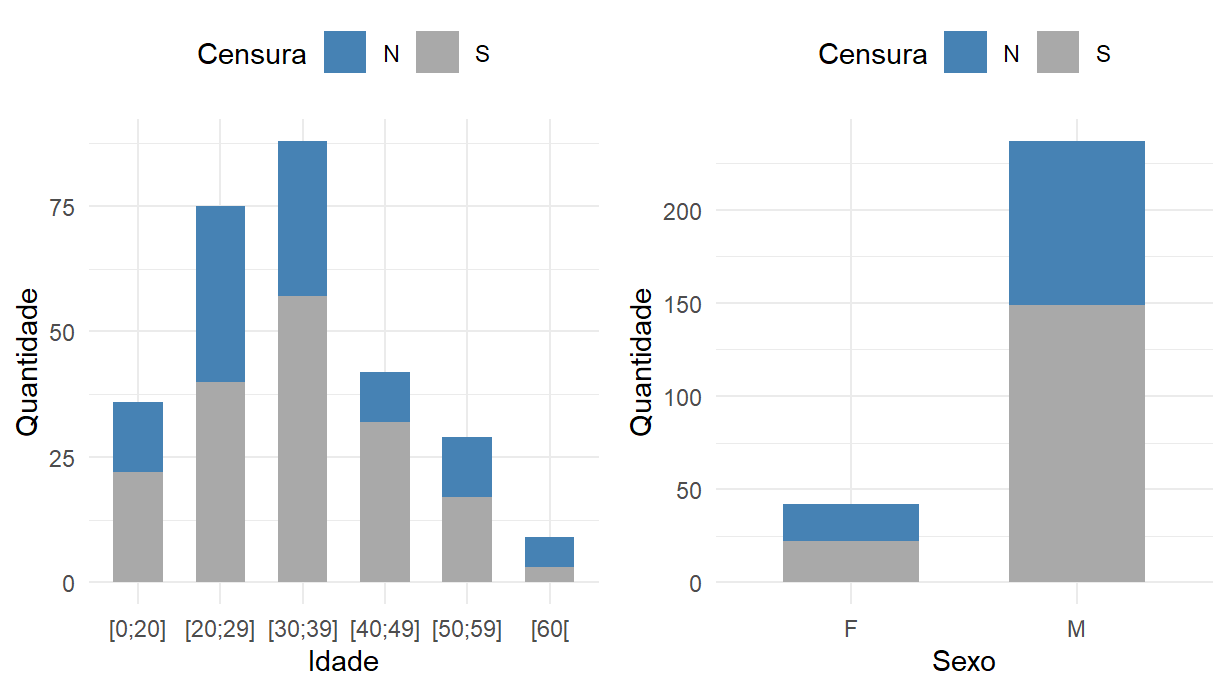
\includegraphics[width=0.8\linewidth]{main_files/figure-latex/fig1-1} 

}

\caption{Distribuição das variáveis Idade e Sexo}\label{fig:fig1}
\end{figure}

Dos 280 indivíduos presentes no estudo, 85,0\% (238/280) eram do sexo masculino e os outros 15\% (42/280) do sexo feminino, no entanto o sexo feminino apresentou maior letalidade se comparada ao sexo masculino, o que pode ser decorrente da baixa quantidade de observações presentes para o sexo feminino.

Em relação a idade, a média dos indivíduos presentes é de 33 anos que também equivale a mediana dos dados. O indivíduo com a menor idade possui 2 anos, enquanto o indivíduo com a maior idade possui 80.

Entre as categorias da variável idade, 32\% (88/280) estão presentes na categoria de indivíduos de 30 a 39 anos, e apenas 3\% (9/280) dos indivíduos do estudo presentes na categoria de 60 ou mais anos de idade.

\begin{figure}[!h]

{\centering 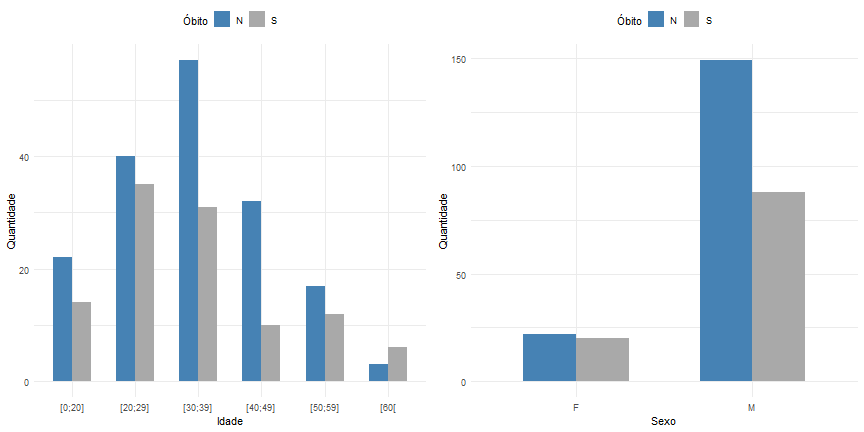
\includegraphics[width=0.8\linewidth]{main_files/figure-latex/fig2-1} 

}

\caption{Distribuição da variável tempo}\label{fig:fig2}
\end{figure}

Quanto a variável resposta tempo, conforme a figura 2, cerca de 88\% (250/280) dos indivíduos apresentam um tempo igual ou inferior a 22 dias. Um ponto interessante de se obervar é o fato de que para um tempo superior a 22 dias, apenas 2 dos 30 indivíduos apresentam censura, ou seja, experimentaram o evento de interesse (óbito).

Outro ponto de atenção é a alta incidência de censura para os tempos iniciais. Cerca de 94\% das censuras registradas aconteceram para tempos iguais ou inferiores à 10, e apenas 1 censura entre os indivíduos com tempo superior a 40.

Para a regional de saúde em que ocorreu o atendimento, olhando a figura 3 União da vitória com 33\% (93/280), foi a regional de saúde com o maior número de ocorrências, e Irati com 16\% (46/280) a com o menor número de ocorrências registradas.

\begin{figure}[!h]

{\centering \includegraphics[width=0.8\linewidth]{main_files/figure-latex/fig3-1} 

}

\caption{Distribuição da variável regional de saúde}\label{fig:fig3}
\end{figure}

Quanto as variáveis relacionadas a sintomas, olhando a tabela 1 conseguimos as frequências absolutas e relativas (percentuais) em cada uma das categiorias, bem como as quantidades de falhas (apresentar o evento de interesse óbito) e censura.

O sintoma que esteve mais presente entre os infectados foi a cefaleia, presente em 242 dos 280 indivíduos, seguido da mialgia em 242.

O sintomas que se mostraram menos presentes foram os sintomas mais extremos. Sinais hemorrágicos com 31 aparições seguido da diarreia em 71 dos 280 indivíduos

\begin{table}[ht]
\centering
\caption{Classes gramaticais das palavras presentes na fala dos indivíduos, considerando os grupos de interesse.} 
\label{tab:classeg}
\begin{tabular}{llrlrrll}
  \hline
Sintomas & Categoria & Freq.Absoluta & Freq.Relativa & Censura & Falha & X & X.1 \\ 
  \hline
Tontura & Sim & 161 & 57,50\% & 171 &   1 &  &  \\ 
   & Não & 119 & 42,50\% &   1 &   1 &  &  \\ 
  Cefaleia & Sim & 242 & 86,43\% &   1 &   1 &  &  \\ 
   & Não &  38 & 13,57\% &   1 &   1 &  &  \\ 
  Sangramento Respiratório & Sim & 123 & 43,93\% &   1 &   1 &  &  \\ 
   & Não & 157 & 56,07\% &   1 &   1 &  &  \\ 
  Dispineia & Sim & 199 & 71,07\% &   1 &   1 &  &  \\ 
   & Não &  81 & 28,93\% &   1 &   1 &  &  \\ 
  Hipotensão & Sim & 148 & 52,86\% &   1 &   1 &  &  \\ 
   & Não & 132 & 47,14\% &   1 &   1 &  &  \\ 
  Mialgia & Sim & 228 & 81,43\% &   1 &   1 &  &  \\ 
   & Não &  52 & 18,57\% &   1 &   1 &  &  \\ 
  Sinais Hemorrágicos & Sim &  31 & 11,07\% &   1 &   1 &  &  \\ 
   & Não & 249 & 88,93\% &   1 &   1 &  &  \\ 
  Diarreia & Sim &  71 & 25,36\% &   1 &   1 &  &  \\ 
   & Não & 209 & 74,64\% &   1 &   1 &  &  \\ 
  Ureia e Creatina & Sim &  91 & 32,50\% &   1 &   1 &  &  \\ 
   & Não & 189 & 67,50\% &   1 &   1 &  &  \\ 
   \hline
\end{tabular}
\end{table}

\hypertarget{considerauxe7uxf5es-finais}{%
\chapter{Considerações Finais}\label{considerauxe7uxf5es-finais}}

\bigskip

Apresente as considerações finais (ou conclusões) do trabalho.

\setlength{\afterchapskip}{\baselineskip}
\bibliography{bib/ref.bib}

\postextual

% ----------------------------------------------------------
% Referências bibliográficas
% ----------------------------------------------------------

% \setlength{\afterchapskip}{\baselineskip}
% \bibliography{}

% ----------------------------------------------------------
% ELEMENTOS PÓS-TEXTUAIS
% ----------------------------------------------------------
% \postextual
% ----------------------------------------------------------


\end{document}
